\documentclass[titlepage, a4paper, 12pt]{article}
\usepackage[swedish]{babel}
\usepackage[utf8]{inputenc}
\usepackage{verbatim}
\usepackage{fancyhdr}
\usepackage{graphicx}
\usepackage{parskip}

% SourceCode
\usepackage{listings}
\usepackage{color}

% Include pdf with multiple pages ex \includepdf[pages=-, nup=2x2]{filename.pdf}
\usepackage[final]{pdfpages}
% Place figures where they should be
\usepackage{float}

% SourceCode
\definecolor{keywordcolor}{rgb}{0.5,0,0.75}
\lstset{
  inputencoding=utf8,
  language=Java,
  extendedchars=true,
  basicstyle=\scriptsize\ttfamily,
  stringstyle=\color{blue},
  commentstyle=\color{red},
  numbers=left,
  firstnumber=auto,
  numberblanklines=true,
  stepnumber=1,
  showstringspaces=false,
  keywordstyle=\color{keywordcolor}
  % identifierstyle=\color{identifiercolor}
}

% Float for text
\floatstyle{ruled}
\newfloat{kod}{H}{lop}
\floatname{kod}{Kodsnutt}

% vars
\def\title{Termiter i NetLogo}
\def\preTitle{Laboration 1}
\def\kurs{Emergenta system, VT-09}

\def\namn{Andreas Jakobsson}
\def\mail{dit06ajs@cs.umu.se}
\def\namnTva{Anton Johansson}
\def\mailTva{dit06ajn@cs.umu.se}

\def\pathtocode{$\sim$dit06ajn/edu/emergenta-system/lab1/src}

\def\handledareEtt{Jonny Pettersson, jonny@cs.umu.se}
\def\handledareTva{Anders Broberg, bopspe@cs.umu.se}

\def\inst{datavetenskap}
\def\dokumentTyp{Laborationsrapport}

\begin{document}
\begin{titlepage}
  \thispagestyle{empty}
  \begin{small}
    \begin{tabular}{@{}p{\textwidth}@{}}
      UMEÅ UNIVERSITET \hfill \today \\
      Institutionen för \inst \\
      \dokumentTyp \\
    \end{tabular}
  \end{small}
  \vspace{10mm}
  \begin{center}
    \LARGE{\preTitle} \\
    \huge{\textbf{\kurs}} \\
    \vspace{10mm}
    \LARGE{\title} \\
    \vspace{15mm}
    \begin{large}
      \namn, \mail \\
      \namnTva, \mailTva\\
      \texttt{\pathtocode}
    \end{large}
    \vfill
    \large{\textbf{Handledare}}\\
    \mbox{\large{\handledareEtt}}
    \mbox{\large{\handledareTva}}
  \end{center}
\end{titlepage}

\newpage
\mbox{}
\vspace{70mm}
\begin{center}
% Dedication goes here
\end{center}
\thispagestyle{empty}
\newpage

\pagestyle{fancy}
\rhead{\today}
\lhead{\footnotesize{\namn, \mail\\\namnTva, \mailTva}}
\chead{}
\lfoot{}
\cfoot{}
\rfoot{}

\cleardoublepage
\newpage
\tableofcontents
\cleardoublepage

% \fancyfoot[LE,RO]{\thepage}
\cfoot{\thepage}
\pagenumbering{arabic}

\section{Problemspecifikation}\label{sec:problemspecifikation}
Laborationen gick ut på att göra ändringar i en befintlig
NetLogo\footnote{http://ccl.northwestern.edu/netlogo/} modell som
imiterar myrors beteende att bygga myrstackar. Ändringarna som skulle
göras och studeras var:

\begin{itemize}
\item Sortering av flera sorters träbitar för att bygga olika
  myrstackar.
\item Laborera med feltolerans, vad händer med modellen om det införs
  myror som på något sätt stör de andra myrornas beteende?
\end{itemize}
% Behövs det ytterligare regler i termiterna för att systemet ska
% konvergera till en separat hög för varje sorts träbitar?

Laborationsspecifikation finns i original på sidan:\\
\verb!http://www.cs.umu.se/kurser/5DV017/VT09/lab/lab1.html!

\section{Reflektioner}
Nedan avsnitt beskriver analysen som gjorts med avseende på frågorna
från problemspecifikationen.

\subsection{Sortering av olika träbitar}
% Reflektion kring er lösning och eventuella begränsningar

% Den ursprungliga termitmodellen innehåller endast en sorts termiter
% och en sorts träbitar. Utöka modellen till minst två sorters termiter
% och två sorters träbitar. Behövs det ytterligare regler i termiterna
% för att systemet ska konvergera till en separat hög för varje sorts
% träbitar? Behövs det ytterligare regler för att minska
% konvergeringstiden? Med konvergering menas här att det endast finns en
% hög av varje sorts träbitar när systemet konvergerat.

För att sortera olika sorters träbitar görs skapas olika myrsorter som
var för sig enbart är intresserade av att plocka upp och lägga ner
träbitar av en specifik sort. För att en myrsort ska lägga ner sin
träbit krävs att den först hittat en träbit av samma sort. Det är
alltså inga ny regler som införts bara nya myrsorter och
träbitar. Myrsorterna är helt oberoende av varandra.

Vid försök med en myrsort som plockar upp alla möjliga träsorter men
enbart lägger ner dem när de hittat en träsort av samma typ som myran
själv bär på blev det problem med att högar bildades av blandade
träsorter. Detta eftersom myrorna inte var benägna att gå in mot
mitten av en hög för att plocka träbitar, så fort en träbit hittades
plockade den och lades så fort en liknande träbit hittades, vilket
alltså gjorde att myrorna alltid höll sig i utkanten av högarna. Ingen
filtrering av redan skapade högar utfördes.

För att minska tiden det tog för myrorna att av varje träsort enbart
bilda en samlad hög ökades stegen som myrorna tog mellan varje
procedur.

\subsection{Feltolerans}
% I ett system är feltolerans en viktig egenskap, ett naturligt eller
% artificiellt system måste tåla i en viss utsträckning att saker går
% fel och att andra agenter i dess omgivning vill förstöra. Studera hur
% termitmodellen reagerar om det införs termiter som på något sätt
% förstör (exempelvis genom att plocka upp träbitar och lägga ned dem
% där inga andra träbitar finns). Frågor att fundera kring är: Hur stor
% andel förstörande termiter behövs det minst för att förstöra
% uppbyggnaden av en hög? Hur påverkas konvergeringshastigheten? Studera
% detta med endast en sorts termiter/träbitar och med flera sorters
% termiter/träbitar.

%  I er inlämnade lösning ska det enkelt gå att ändra antalet av
%  respektive sort termiter och andelen av respektive sort träbitar.

För att testa feltoleransen i systemet lades myror in som plockar upp
alla träsorter de stöter på och efter ett bestämt antal steg försöker
lägga ner denna träbit på en ledig plats.

Test gjordes där kvoten mellan jobbande myror och förstörande myror
varierades.  I figur \ref{fig:first-conv-pic} –
\ref{fig:last-conv-pic} har kvoten förstörande myror varierats mellan
0 till 10 \%, konvergering av högarna påbörjas inom 90 sekunder. Ökas
kvoten till 12 \% syns inga tecken på konvergering av högarna inom 180
sekunder, se figur \ref{fig:12proc}. Detta kan tänkas beror på att
antalet myror av båda sorter i förhållande till storleken på miljön de
befinner sig i har blivit för fylld. Troligtvis kommer även denna
modell att konvergera om den låtes köra vidare.

Vidare tester gjordes med ett mindre antal myror fast med samma
densitet av träbitar (totalt 400 arbetande myror + varierat antal
förstörande myror). Figur \ref{fig:first-new} - \ref{fig:last-new}
visar att modellerna med högre kvot förstörande myror även de
konvergerar vid längre körningar. En krans av spridda träbitar runt
högarna tyder på den kontinuerliga förstörelsen.

Vi antar att det kommer att krävas fler antal förstörande myror än
antalet uppbyggande myror för att hindra konvergering av högarna. Ett
test av detta skulle ta allt för lång tid att genomföra.

I de gjorda testen konvergerar högarna alltid men konvergeringstiden
ökar markant.

\begin{figure}
  \begin{minipage}[b]{0.5\linewidth} % A minipage that covers half the page
    \centering
    \caption{30 sekunder, inga badAnts}\label{fig:first-conv-pic}
    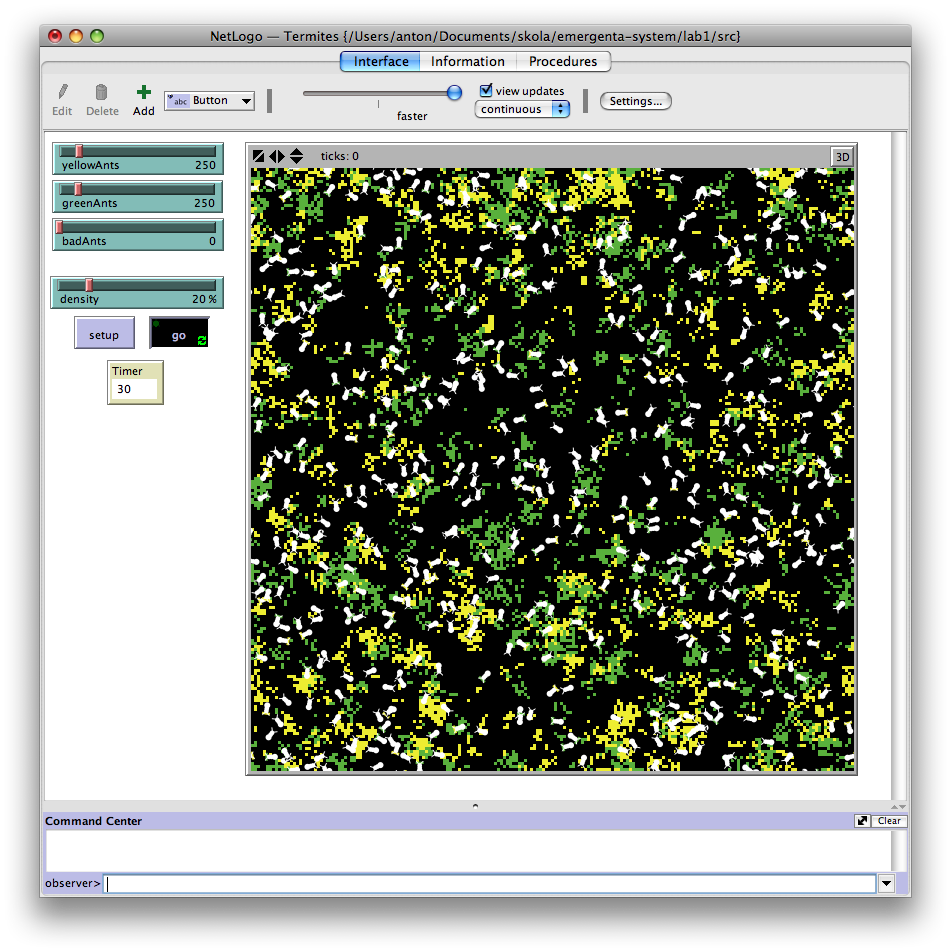
\includegraphics[width=6cm]{images/no-bad-30.png}
  \end{minipage}
  \hspace{0.5cm} % To get a little bit of space between the figures
  \begin{minipage}[b]{0.5\linewidth}
    \centering
    \caption{30 sekunder, 0,02 \% badAnts}
    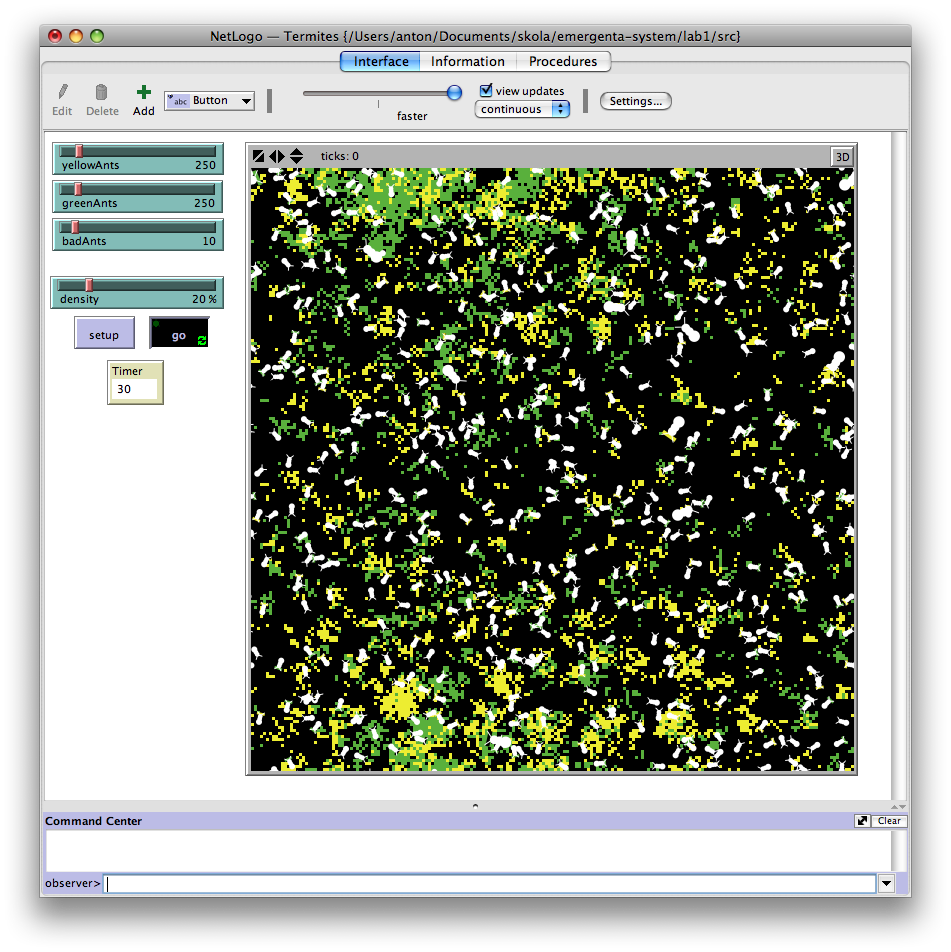
\includegraphics[width=6cm]{images/10-bad-30.png}
  \end{minipage}

  \begin{minipage}[b]{0.5\linewidth} % A minipage that covers half the page
    \centering
    \caption{60 sekunder, inga badAnts}
    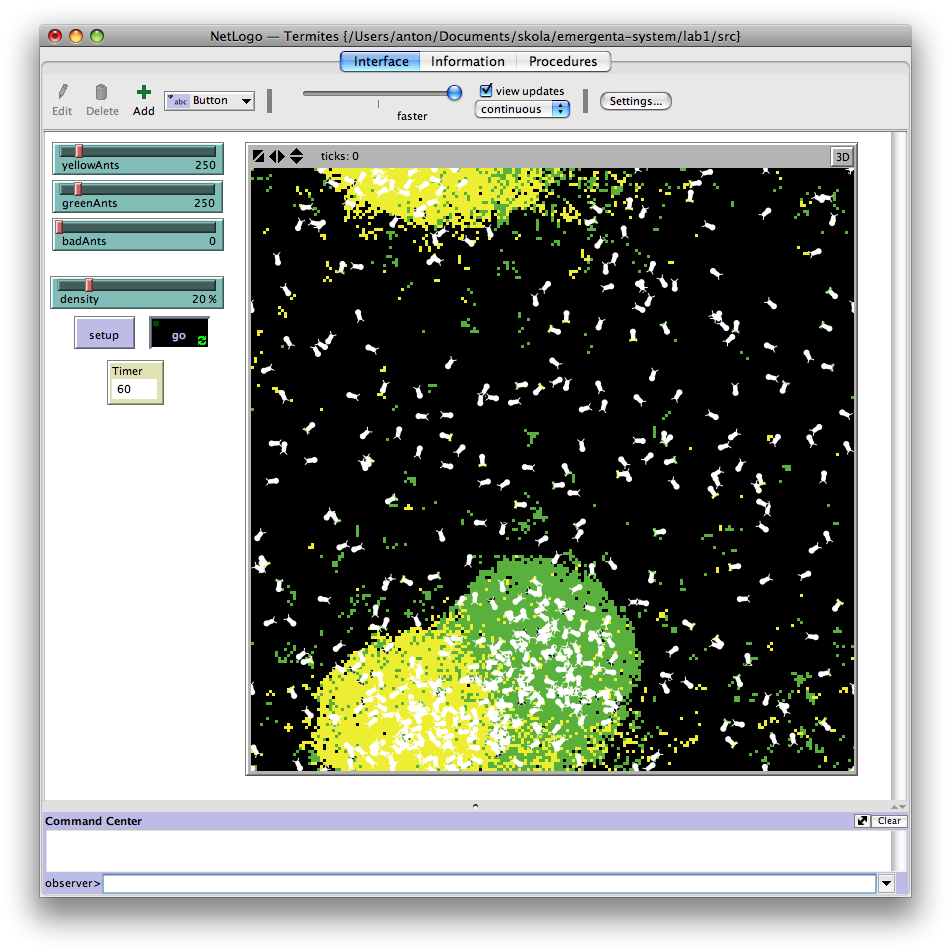
\includegraphics[width=6cm]{images/no-bad-60.png}
  \end{minipage}
  \hspace{0.5cm} % To get a little bit of space between the figures
  \begin{minipage}[b]{0.5\linewidth}
    \centering
    \caption{60 sekunder, 0,02 \% badAnts}
    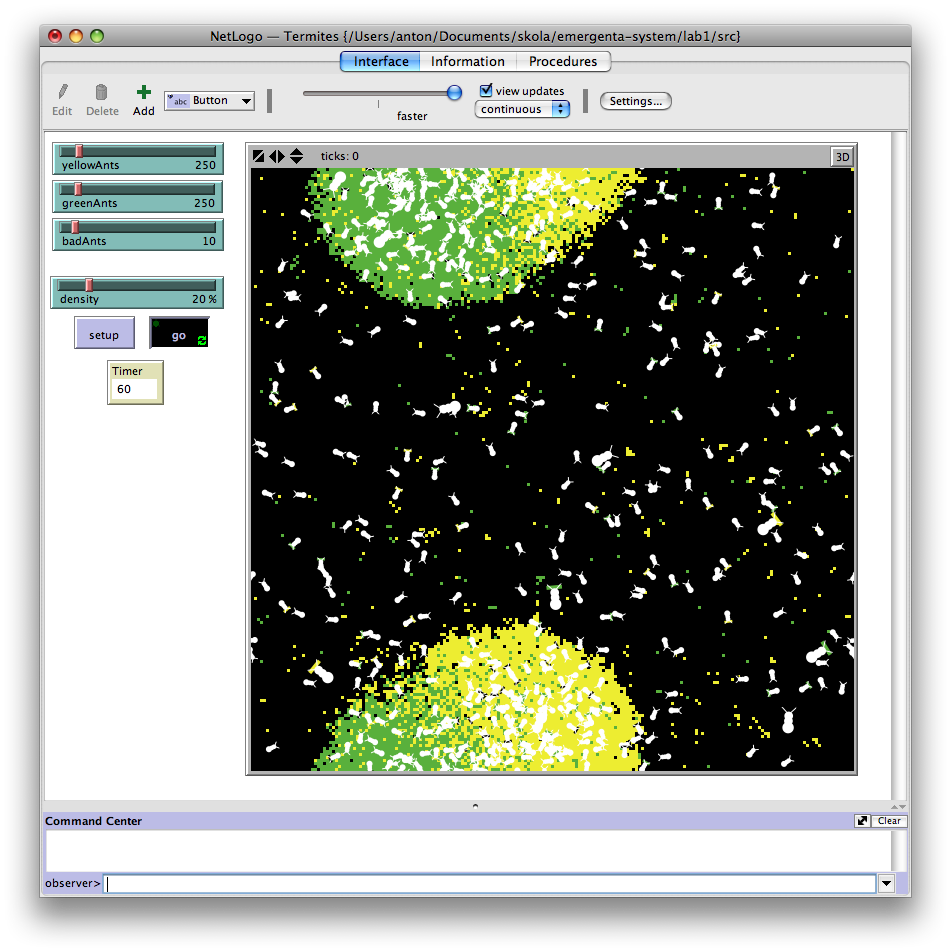
\includegraphics[width=6cm]{images/10-bad-60.png}
  \end{minipage}
  
  \begin{minipage}[b]{0.5\linewidth} % A minipage that covers half the page
    \centering
    \caption{90 sekunder, inga badAnts}
    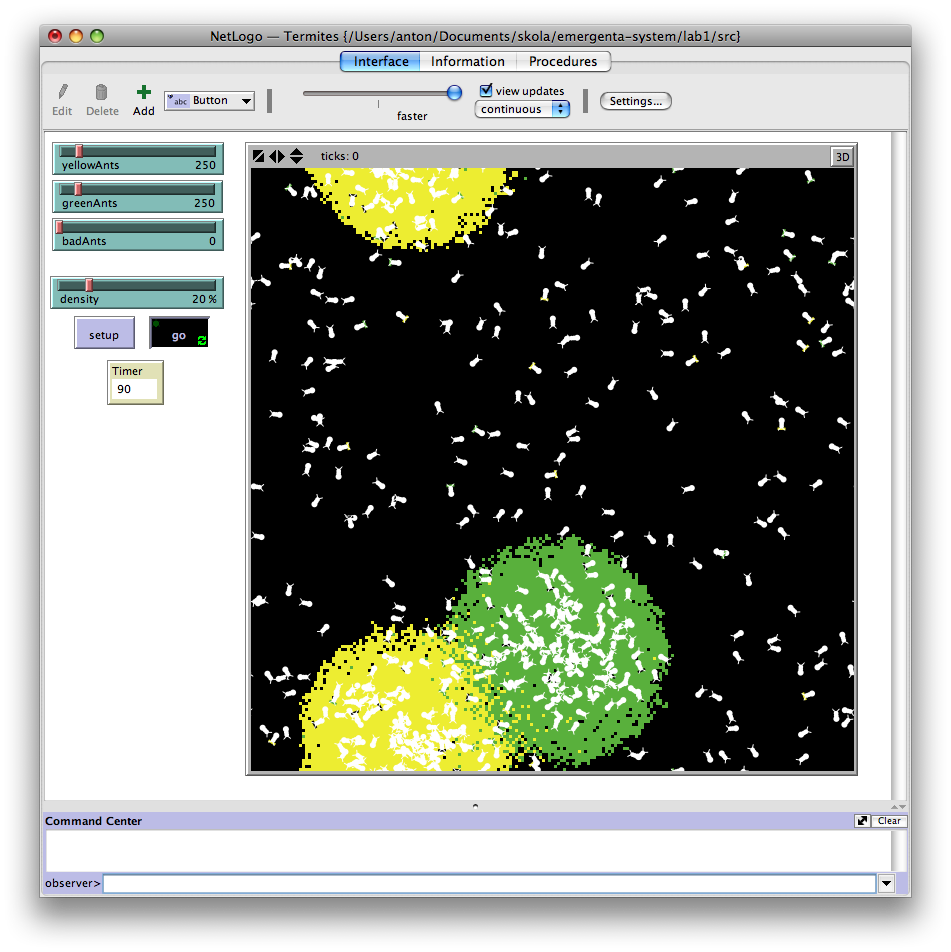
\includegraphics[width=6cm]{images/no-bad-90.png}
  \end{minipage}
  \hspace{0.5cm} % To get a little bit of space between the figures
  \begin{minipage}[b]{0.5\linewidth}
    \centering
    \caption{90 sekunder, 0,02 \% badAnts}
    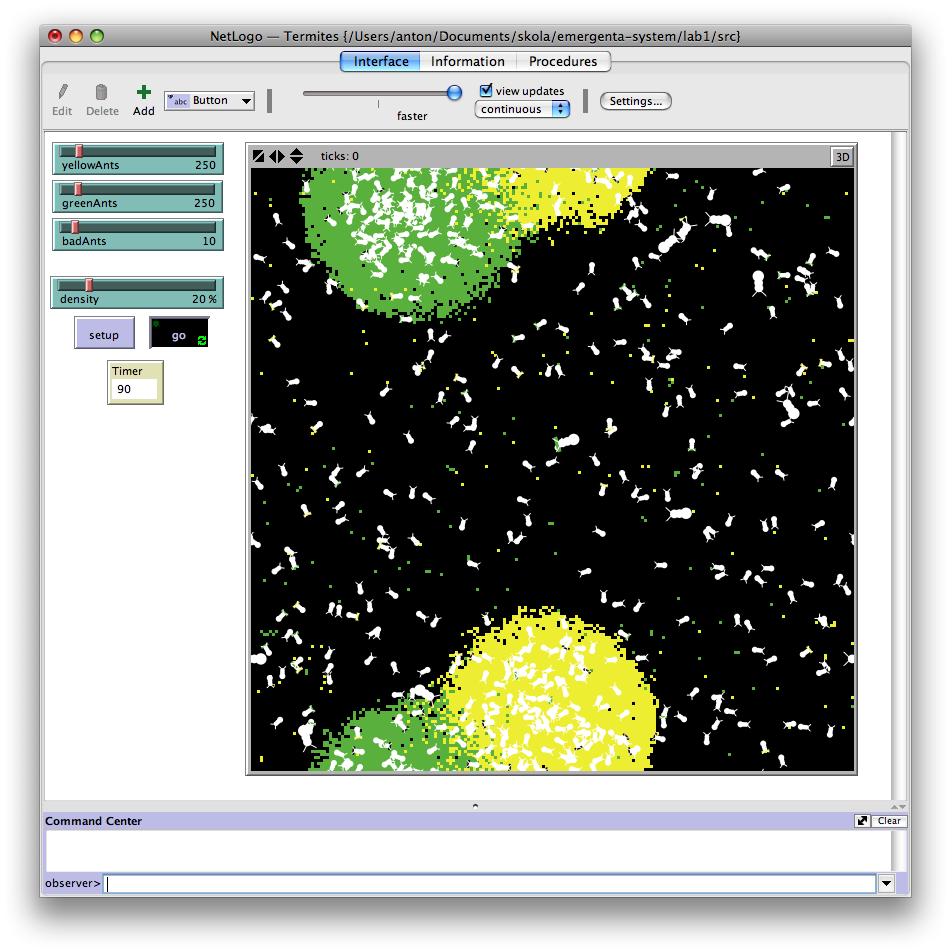
\includegraphics[width=6cm]{images/10-bad-90.png}
  \end{minipage}
\end{figure}

\begin{figure}
  \begin{minipage}[b]{0.5\linewidth} % A minipage that covers half the page
    \centering
    \caption{30 sekunder, 4 \% badAnts}
    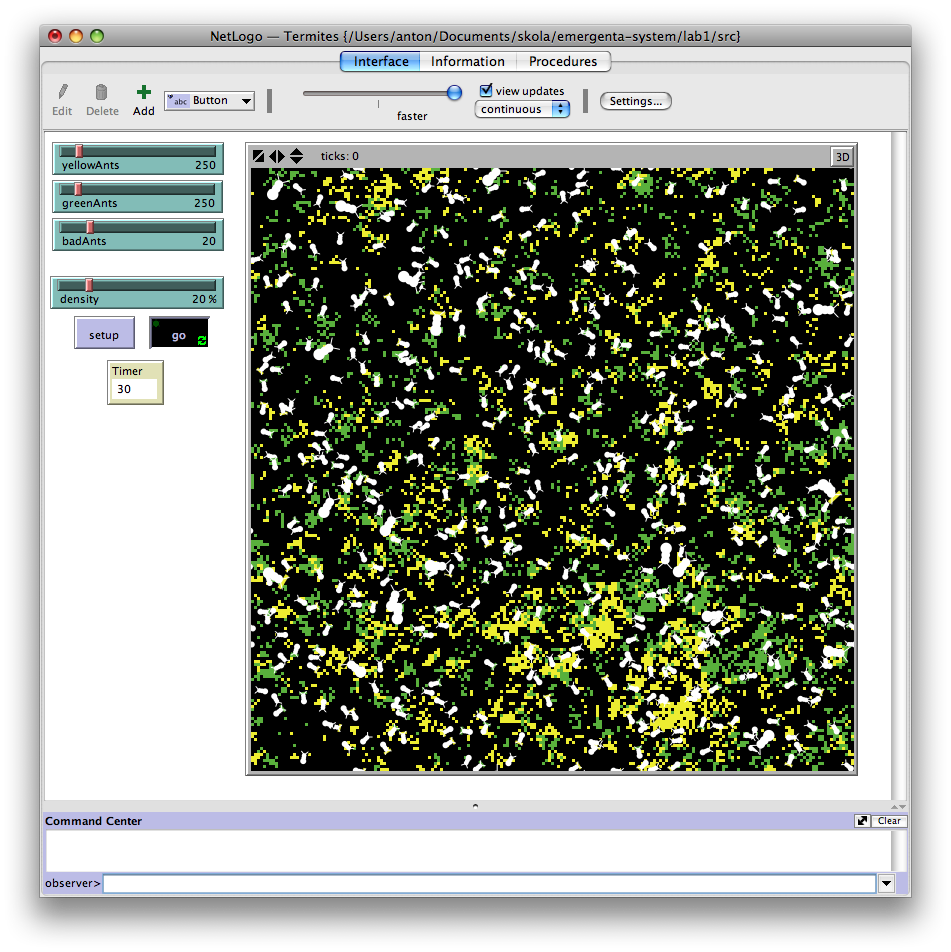
\includegraphics[width=6cm]{images/20-bad-30.png}
  \end{minipage}
  \hspace{0.5cm} % To get a little bit of space between the figures
  \begin{minipage}[b]{0.5\linewidth}
    \centering
    \caption{30 sekunder, 6 \% badAnts}
    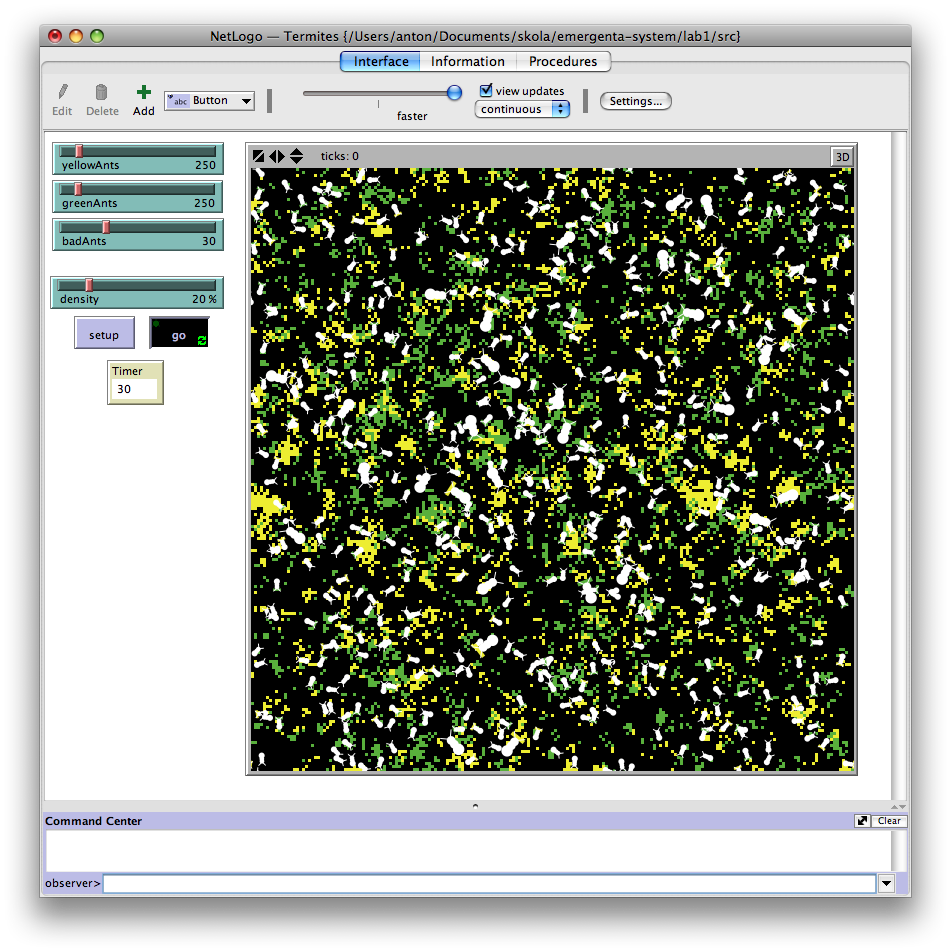
\includegraphics[width=6cm]{images/30-bad-30.png}
  \end{minipage}

  \begin{minipage}[b]{0.5\linewidth} % A minipage that covers half the page
    \centering
    \caption{60 sekunder, 4 \% badAnts}
    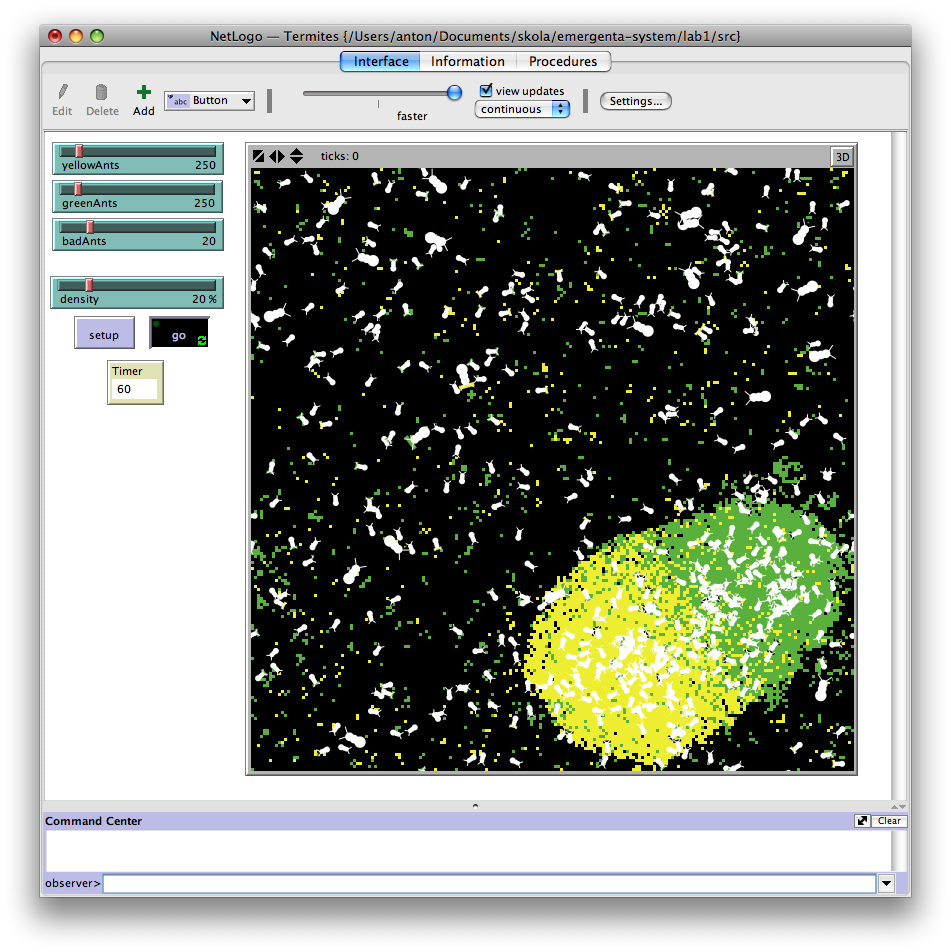
\includegraphics[width=6cm]{images/20-bad-60.png}
  \end{minipage}
  \hspace{0.5cm} % To get a little bit of space between the figures
  \begin{minipage}[b]{0.5\linewidth}
    \centering
    \caption{60 sekunder, 6 \% badAnts}
    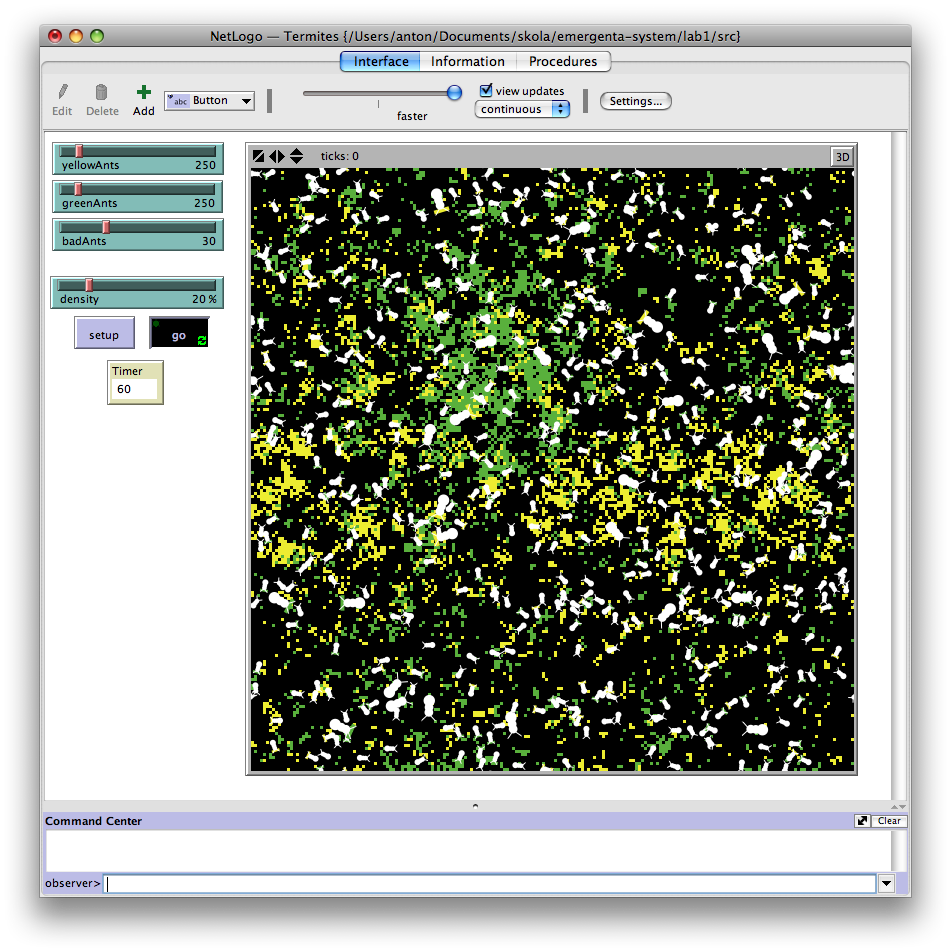
\includegraphics[width=6cm]{images/30-bad-60.png}
  \end{minipage}
  
  \begin{minipage}[b]{0.5\linewidth} % A minipage that covers half the page
    \centering
    \caption{90 sekunder, 4 \% badAnts}
    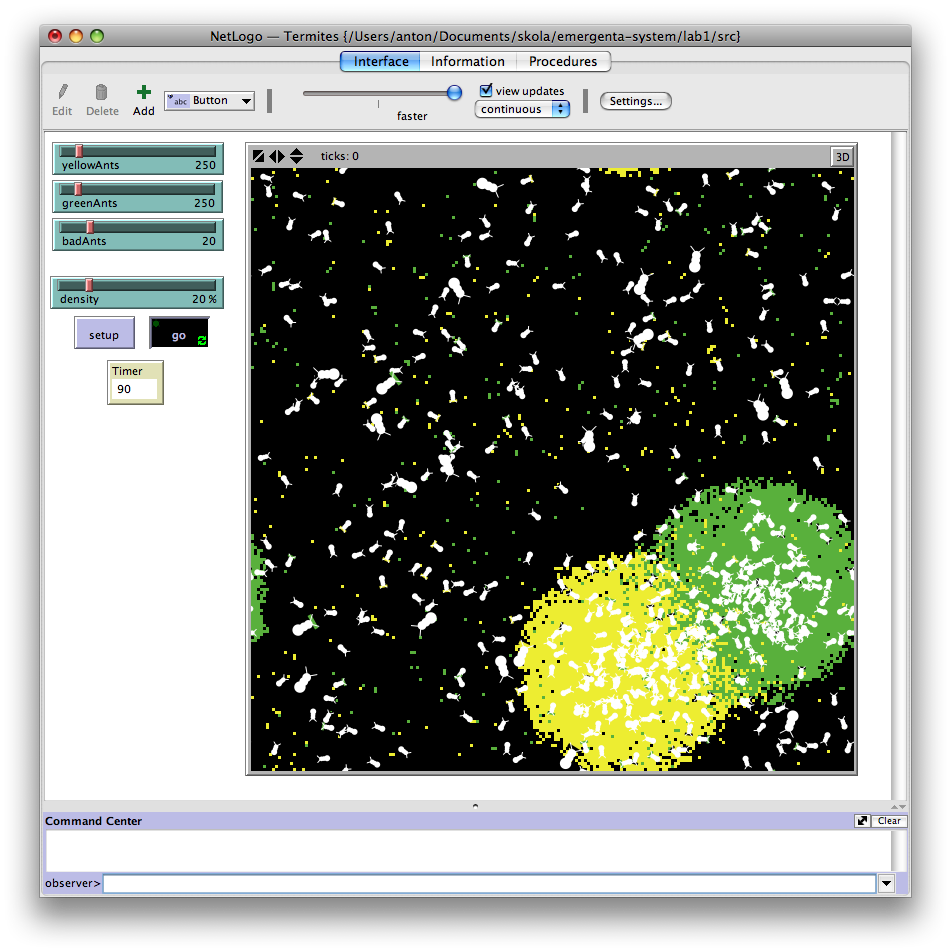
\includegraphics[width=6cm]{images/20-bad-90.png}
  \end{minipage}
  \hspace{0.5cm} % To get a little bit of space between the figures
  \begin{minipage}[b]{0.5\linewidth}
    \centering
    \caption{90 sekunder, 6 \% badAnts}
    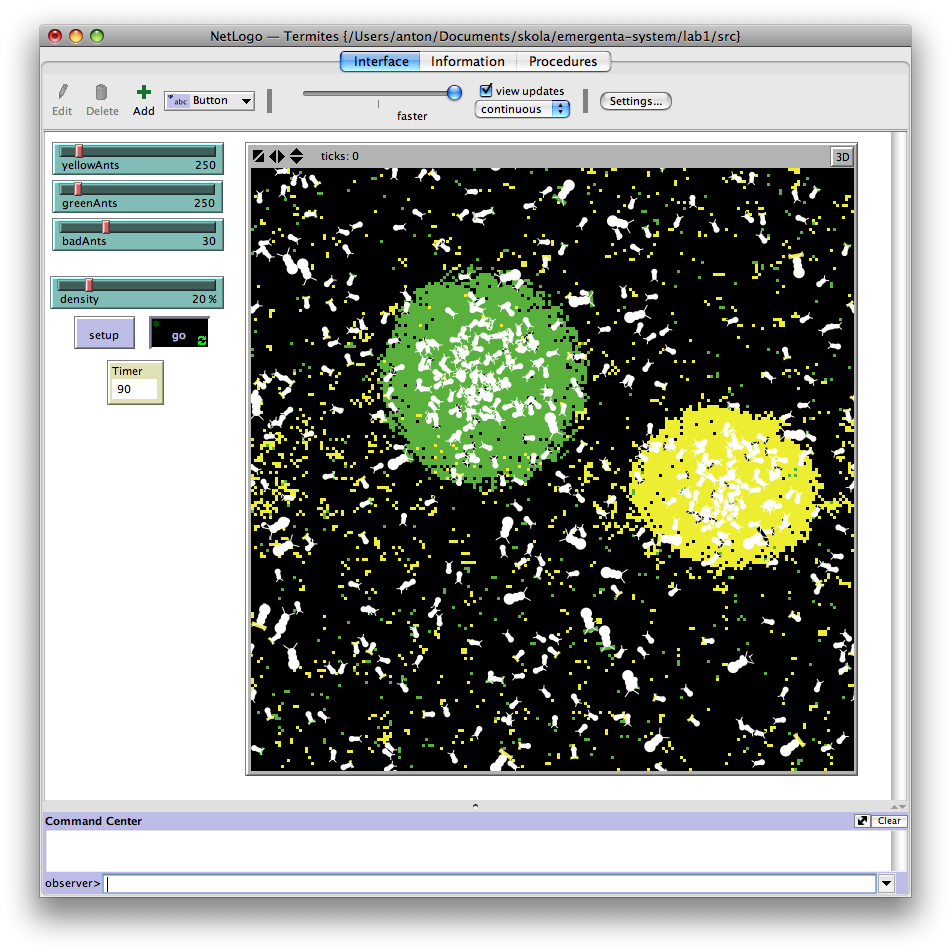
\includegraphics[width=6cm]{images/30-bad-90.png}
  \end{minipage}
\end{figure}

\begin{figure}
  \begin{minipage}[b]{0.5\linewidth} % A minipage that covers half the page
    \centering
    \caption{30 sekunder, 8 \% badAnts}
    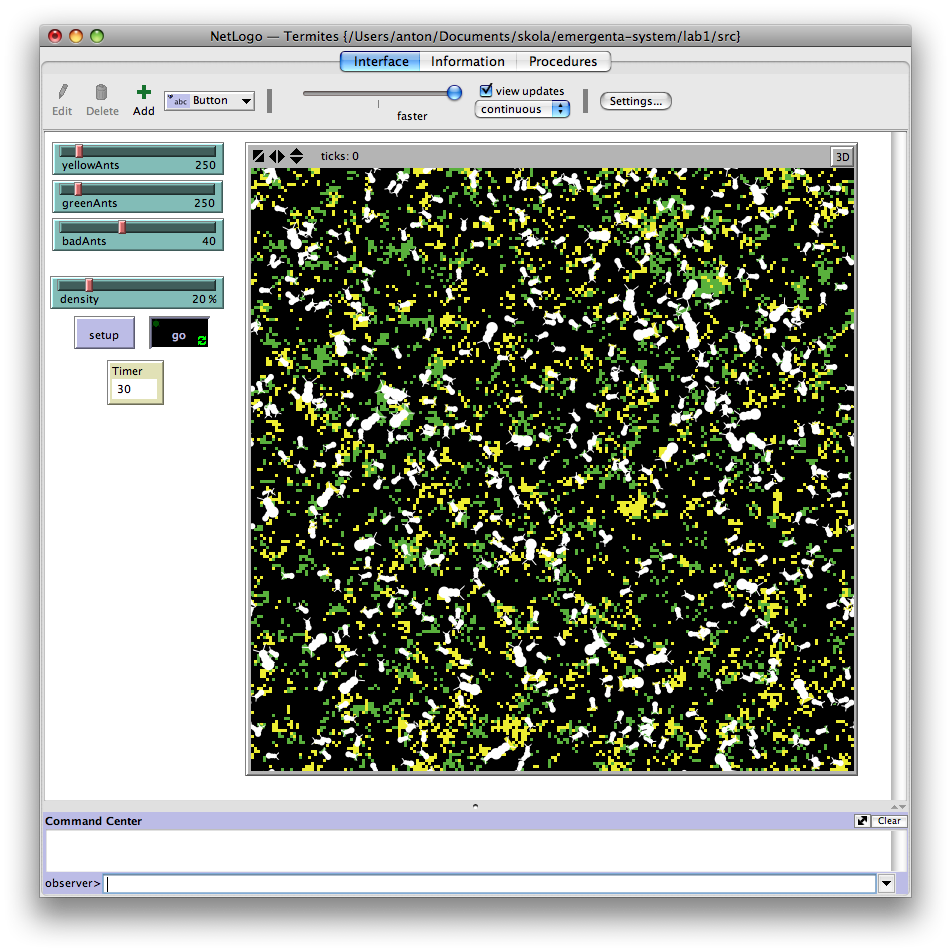
\includegraphics[width=6cm]{images/40-bad-30.png}
  \end{minipage}
  \hspace{0.5cm} % To get a little bit of space between the figures
  \begin{minipage}[b]{0.5\linewidth}
    \centering
    \caption{30 sekunder, 10 \% badAnts}
    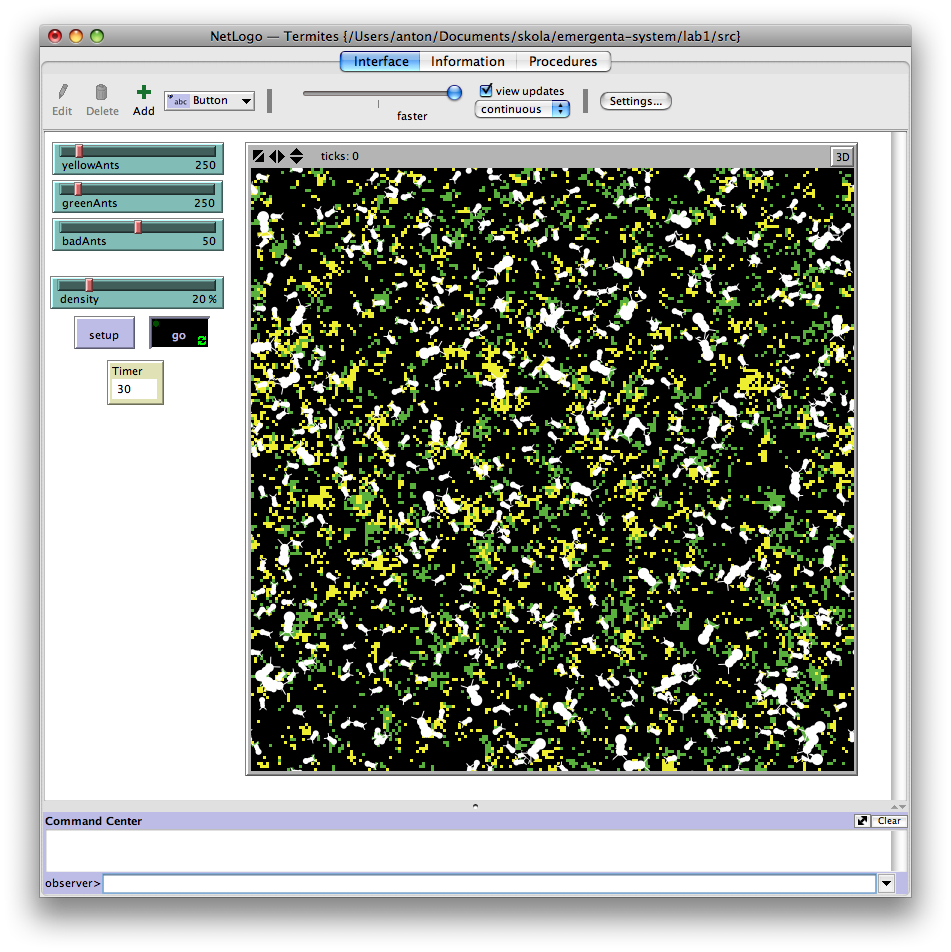
\includegraphics[width=6cm]{images/50-bad-30.png}
  \end{minipage}

  \begin{minipage}[b]{0.5\linewidth} % A minipage that covers half the page
    \centering
    \caption{60 sekunder, 8 \% badAnts}
    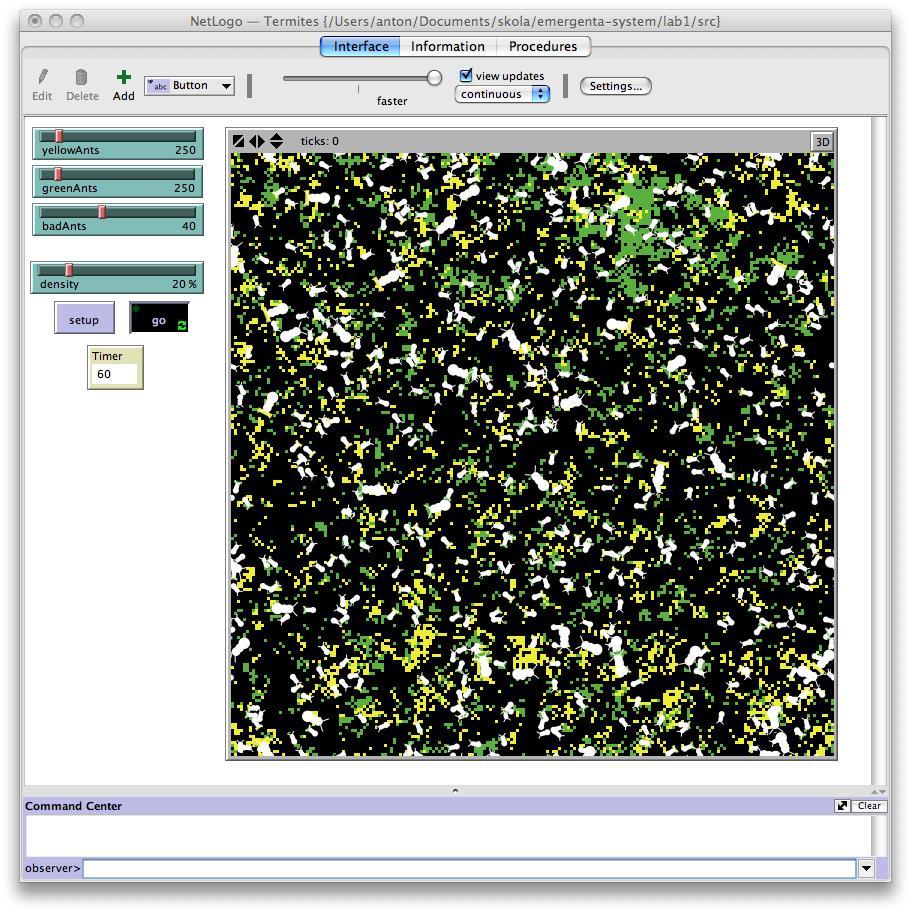
\includegraphics[width=6cm]{images/40-bad-60.png}
  \end{minipage}
  \hspace{0.5cm} % To get a little bit of space between the figures
  \begin{minipage}[b]{0.5\linewidth}
    \centering
    \caption{60 sekunder, 10 \% badAnts}
    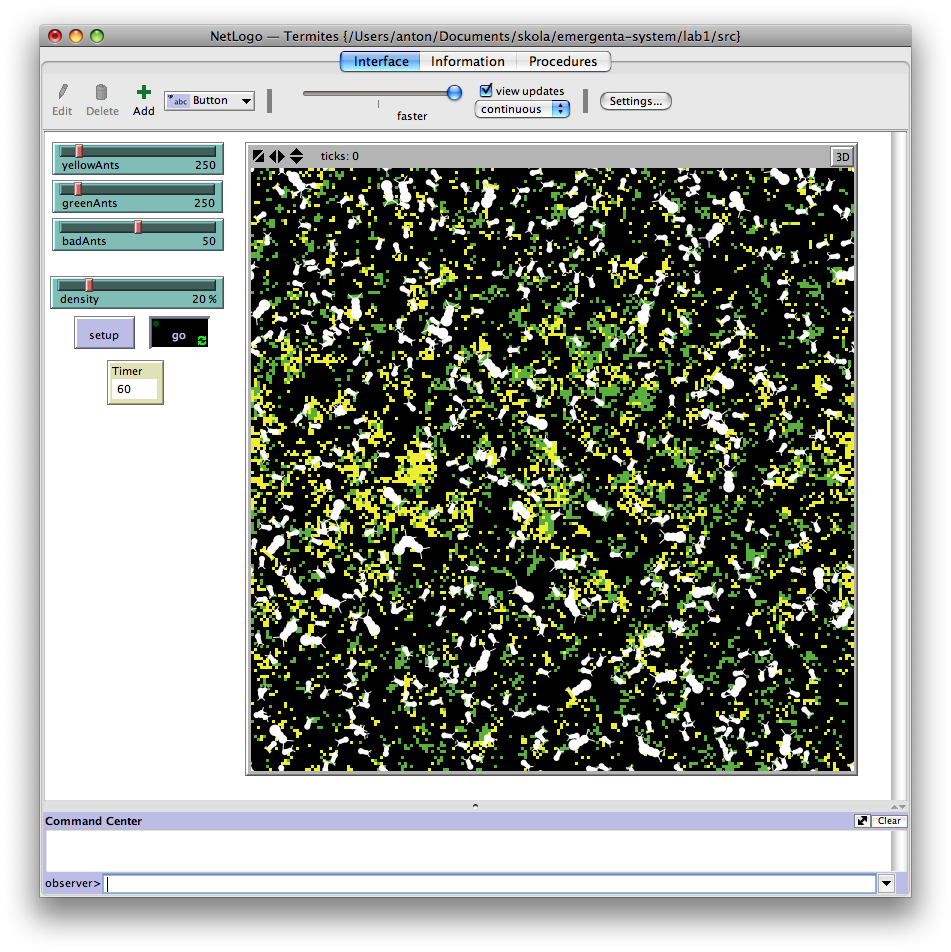
\includegraphics[width=6cm]{images/50-bad-60.png}
  \end{minipage}
  
  \begin{minipage}[b]{0.5\linewidth} % A minipage that covers half the page
    \centering
    \caption{90 sekunder, 8 \% badAnts}
    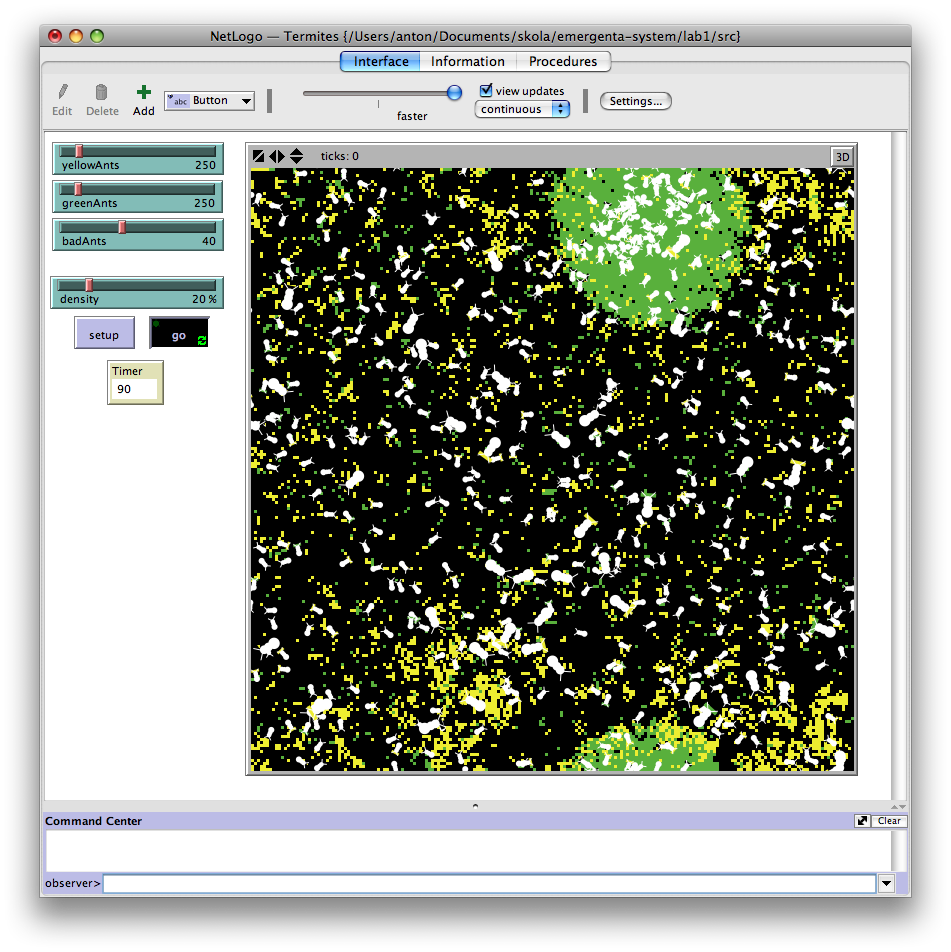
\includegraphics[width=6cm]{images/40-bad-90.png}
  \end{minipage}
  \hspace{0.5cm} % To get a little bit of space between the figures
  \begin{minipage}[b]{0.5\linewidth}
    \centering
    \caption{90 sekunder, 10 \% badAnts}\label{fig:last-conv-pic}
    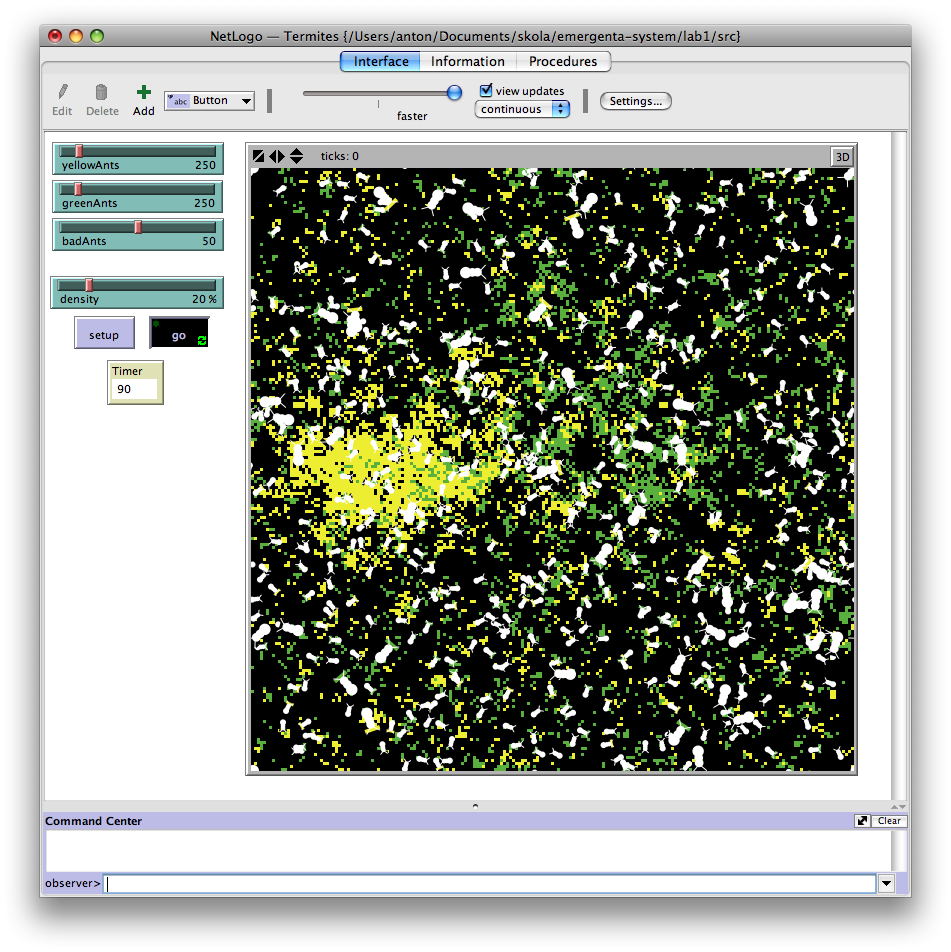
\includegraphics[width=6cm]{images/50-bad-90.png}
  \end{minipage}
\end{figure}

\begin{figure}
  \begin{minipage}[b]{0.5\linewidth} % A minipage that covers half the page
    \centering
    \caption{30 sekunder, 12 \% badAnts}
    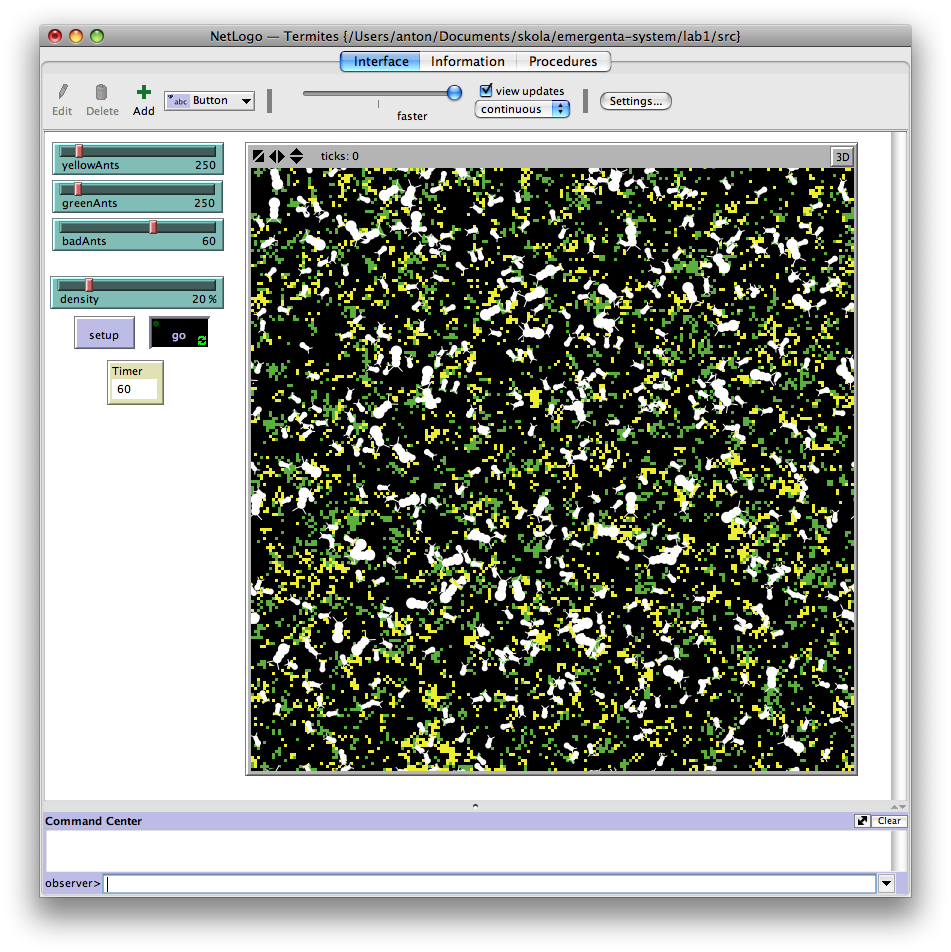
\includegraphics[width=6cm]{images/60-bad-60.png}
  \end{minipage}
  \hspace{0.5cm} % To get a little bit of space between the figures
  \begin{minipage}[b]{0.5\linewidth}
    \centering
    \caption{60 sekunder, 12 \% badAnts}
    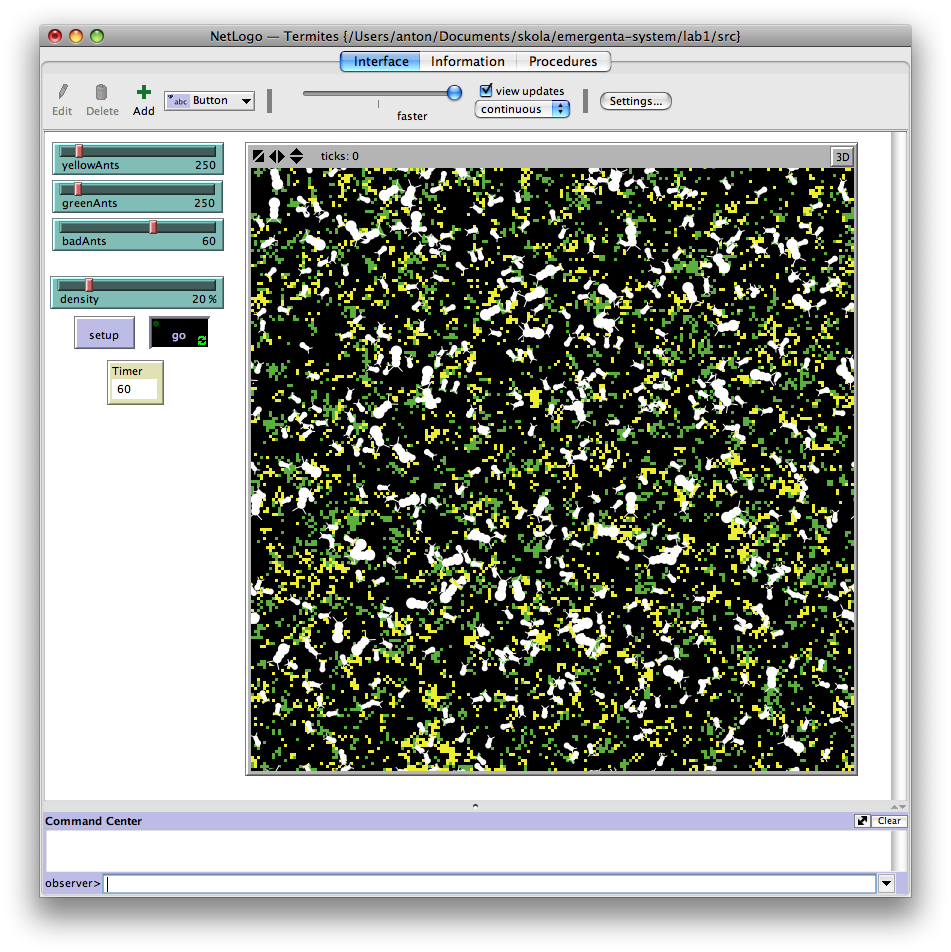
\includegraphics[width=6cm]{images/60-bad-60.png}
  \end{minipage}

  \begin{minipage}[b]{0.5\linewidth} % A minipage that covers half the page
    \centering
    \caption{90 sekunder, 12 \% badAnts}
    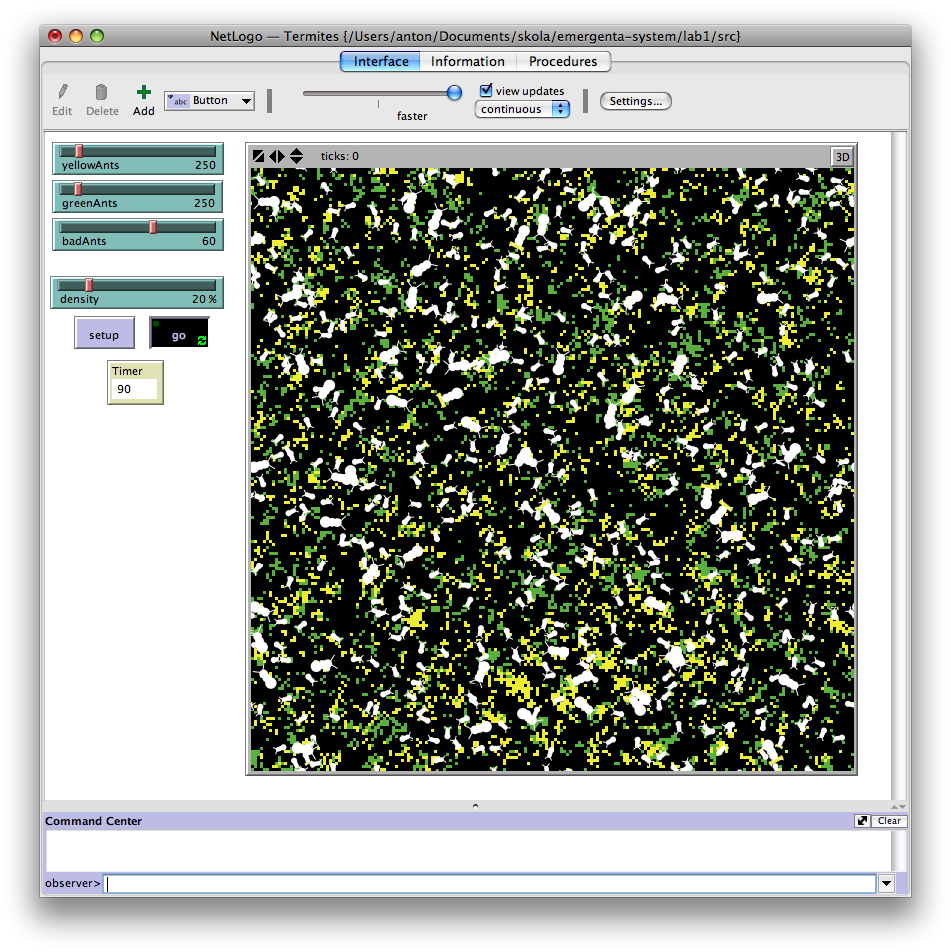
\includegraphics[width=6cm]{images/60-bad-90.png}
  \end{minipage}
  \hspace{0.5cm} % To get a little bit of space between the figures
  \begin{minipage}[b]{0.5\linewidth}
    \centering
    \caption{120 sekunder, 12 \% badAnts}
    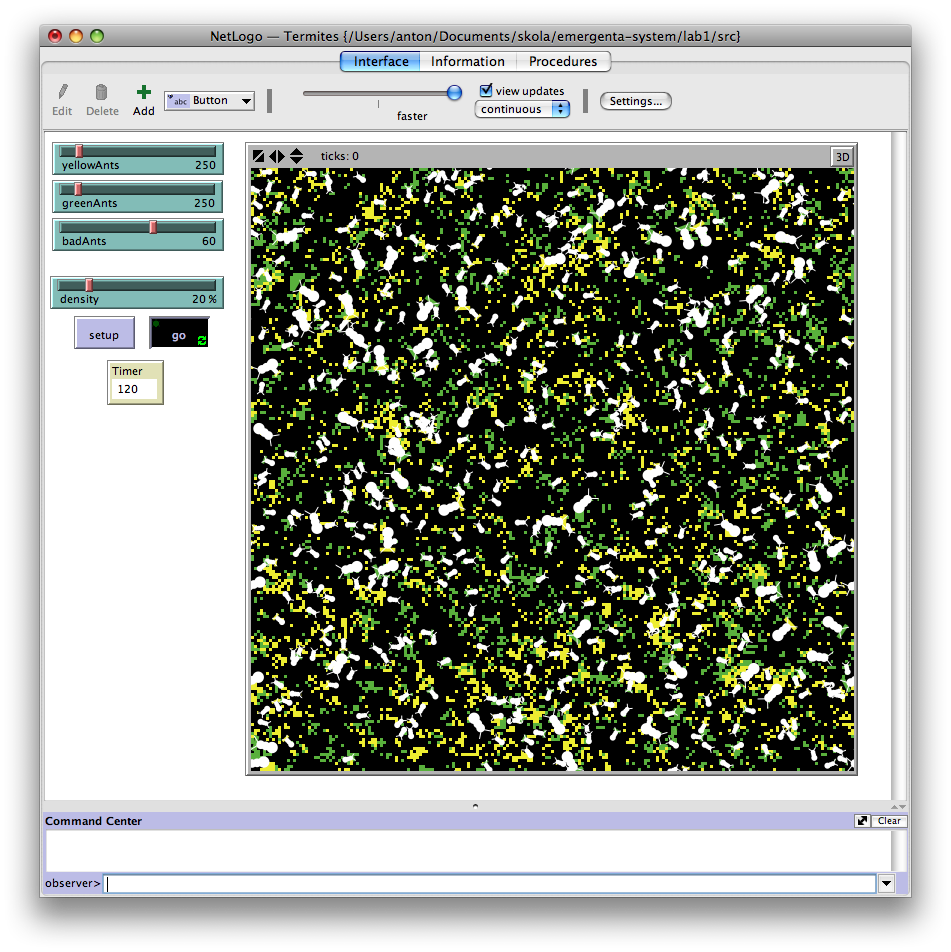
\includegraphics[width=6cm]{images/60-bad-120.png}
  \end{minipage}
  
  \begin{minipage}[b]{0.5\linewidth} % A minipage that covers half the page
    \centering
    \caption{150 sekunder, 12 \% badAnts}
    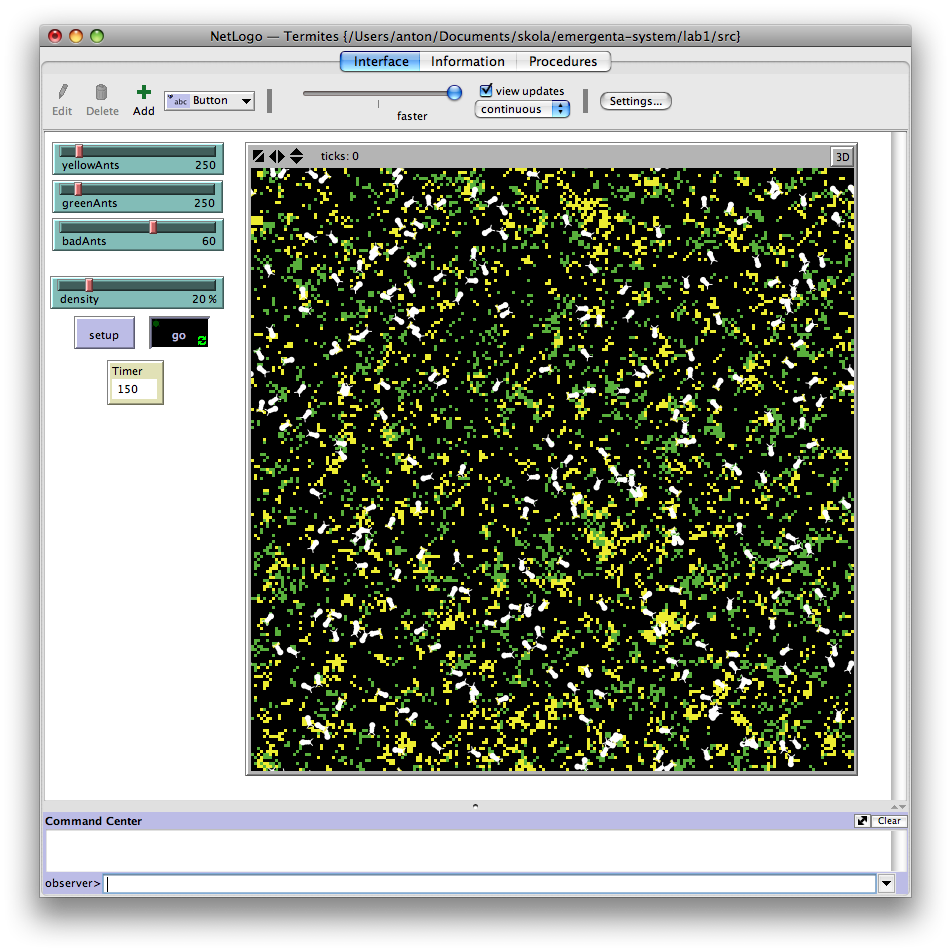
\includegraphics[width=6cm]{images/60-bad-150.png}
  \end{minipage}
  \hspace{0.5cm} % To get a little bit of space between the figures
  \begin{minipage}[b]{0.5\linewidth}
    \centering
    \caption{180 sekunder, 12 \% badAnts}\label{fig:12proc}
    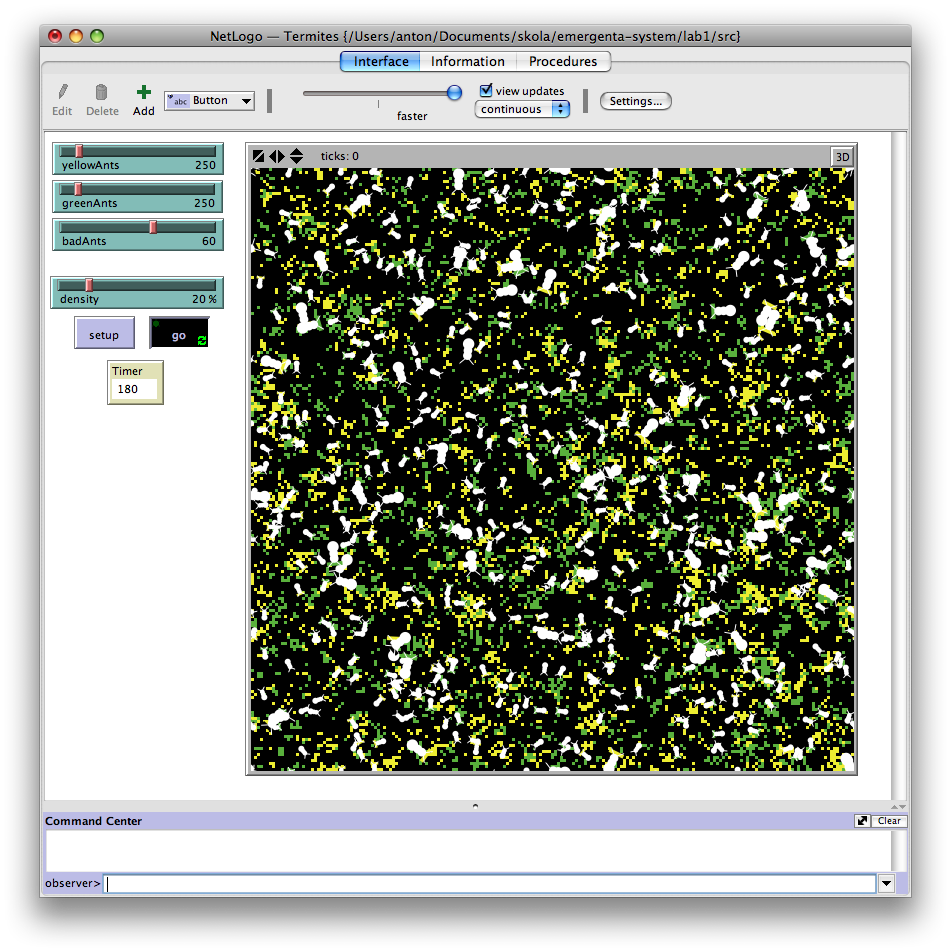
\includegraphics[width=6cm]{images/60-bad-180.png}
  \end{minipage}
\end{figure}


% Nya tester
\begin{figure}
  \begin{minipage}[b]{0.5\linewidth}
    \centering
    \caption{150 sekunder, 20 \% badAnts}\label{fig:first-new}
    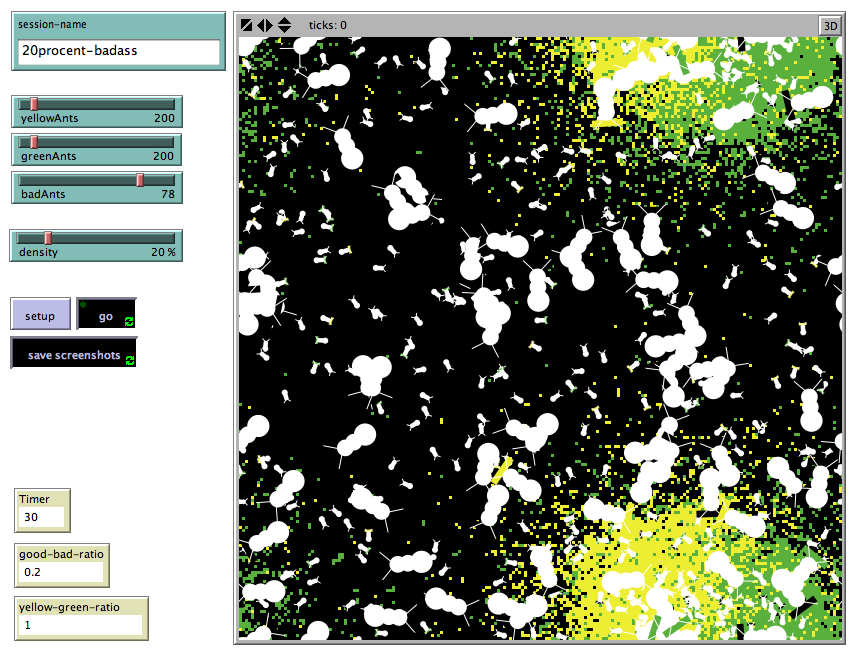
\includegraphics[width=6cm]{images/20procent-badass-150.png}
  \end{minipage}
  \begin{minipage}[b]{0.5\linewidth} % A minipage that covers half the page
    \centering
    \caption{330 sekunder, 30 \% badAnts}
    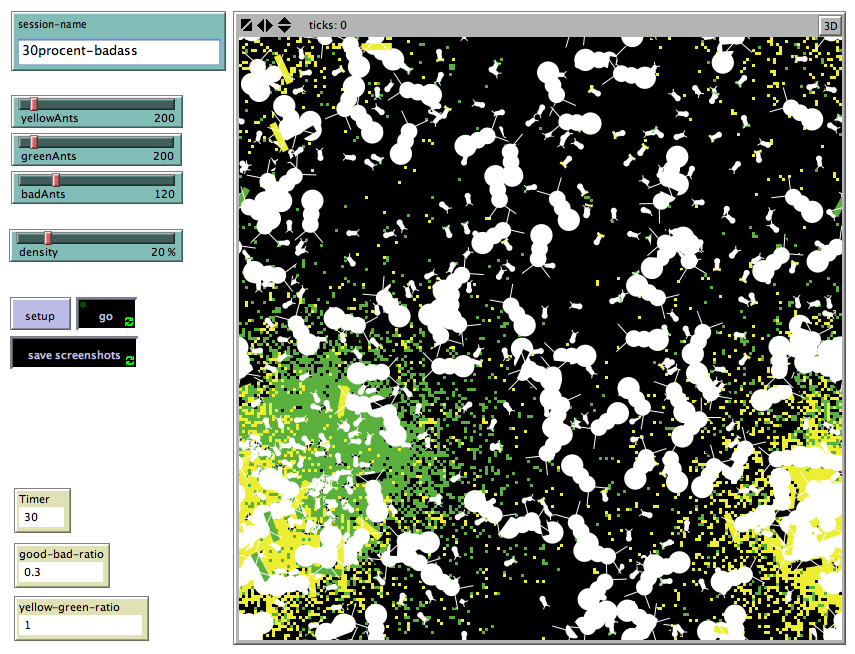
\includegraphics[width=6cm]{images/30procent-badass-330.png}
  \end{minipage}
  \hspace{0.5cm} % To get a little bit of space between the figures
  
  \begin{minipage}[b]{0.5\linewidth} % A minipage that covers half the page
    \centering
    \caption{1320 sekunder, 40 \% badAnts}\label{fig:last-new}
    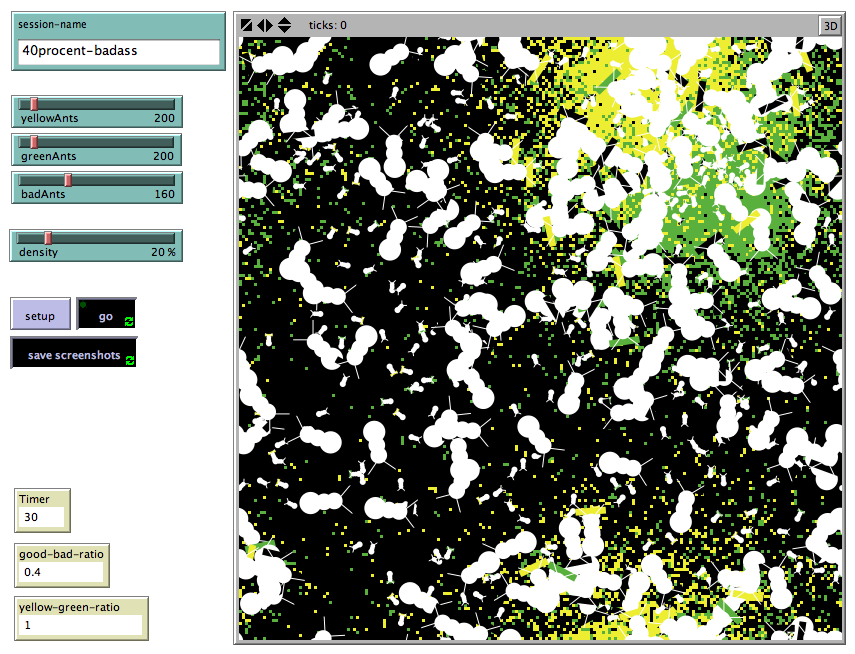
\includegraphics[width=6cm]{images/40procent-badass-1320.png}
  \end{minipage}
  \hspace{0.5cm} % To get a little bit of space between the figures
  
  
  
\end{figure}

\section{Applikationsområden}
% Diskutera de frågor som nämns ovan och försöka att sätta in
% laborationen i ett större sammanhang. Kan du se några
% applikationsområden för den här typen av algoritmer? Kan modellen
% utökas för att göras mer intressant?

Tänkta applikationer för denna typen av algoritmer kan vara till
exempel olika mediciner och behandlingar på nano-nivå där mycket enkla
små agenter gemensamt kan konvergera till en komplex behandlingsform.

Kluster av billiga datorer kan jobba gemensamt för att bilda ett
komplext beteende. Distribuerad bearbetning och lagring av data på
datorer runt om världen. Exempel på sådana projekt är exempel
lösningar som räknar fram stora primtal eller behandlar signaler och
letar efter tecken på utomjordiskt liv.

\newpage
\appendix
\pagenumbering{roman}
\section{Källkod}\label{sec:kallkod}
% Källkoden ska finnas tillgänglig i er hemkatalog
% ~/edu/apjava/lab1/. Bifoga även utskriven källkod.
Härefter följer utskrifter från källkoden och andra filer som hör till
denna laboration

\subsection{Termites.nlogo}\label{Termites.nlogo}
\begin{footnotesize}
  \verbatiminput{../src/Termites.nlogo}
\end{footnotesize}
\end{document}
